\documentclass[aspectratio=169]{beamer}

\usepackage{amsmath}
\usepackage{amssymb}
\usepackage{mathtools}
\usepackage{graphicx}

\usetheme{Madrid}
\usecolortheme{default}
\setbeamertemplate{navigation symbols}{}

\title[]{
Dupire v.s. Neural Networks Delta Hedging}
\subtitle{Erdos Project}
\author{Oscar Arevalo, Alec Hewitt, Ziqing Zhang}
\date{\today}

\begin{document}

\begin{frame}
  \titlepage
\end{frame}

\begin{frame}{Overview}
\begin{itemize}
    \item Dupire model: Why constant volatility is insufficient and how local volatility uses the implied volatility surface.
    \item Neural network approach: How a learning-based method approximates option hedging behavior from market features.
    \item Results and comparison: How the Dupire and neural-network hedges perform in the backtest.
\end{itemize}
\end{frame}

\begin{frame}{Motivation: Beyond Black--Scholes}
  \begin{itemize}
    \item Black--Scholes dynamics:
    \[
      dS_t = rS_t\,dt + \sigma S_t\,dW_t .
    \]
    \item However, in reality volatilities vary across strikes and maturities:
    \[
      \sigma_{\mathrm{imp}} = \sigma_{\mathrm{imp}}(K,T).
    \]
    \item This implied volatility surface shows that one constant $\sigma$ cannot fit all traded option prices.
    \item Dupire starts from this market surface and asks how to build a dynamic model consistent with it.
  \end{itemize}
\end{frame}

\begin{frame}{Dupire Local Volatility}
  \begin{itemize}
    \item Replace constant volatility with a state- and time-dependent function:
    \[
      dS_t = rS_t\,dt + \sigma_{\mathrm{loc}}(S_t,t)S_t\,dW_t .
    \]
    \item Financially, $\sigma_{\mathrm{loc}}(S,t)$ is the instantaneous volatility assigned to state $(S,t)$.
    \item Let $C(K,T)$ be the time-0 price of a European call with strike $K$ and maturity $T$.
    \item Dupire's formula recovers local variance from derivatives of the call price surface:
    \[
      \sigma_{\mathrm{loc}}^2(K,T)
      =
      \frac{\frac{\partial C}{\partial T}
      + rK\frac{\partial C}{\partial K}}
      {\frac{1}{2}K^2\frac{\partial^2 C}{\partial K^2}}.
    \]
    \item Here $C$ is the call price, $K$ is strike, $T$ is maturity, and $r$ is the risk-free rate.
  \end{itemize}
\end{frame}

\begin{frame}{From Implied to Local Volatility}
  \centering
  \begin{columns}[c,onlytextwidth]
    \begin{column}{0.38\textwidth}
      \centering
      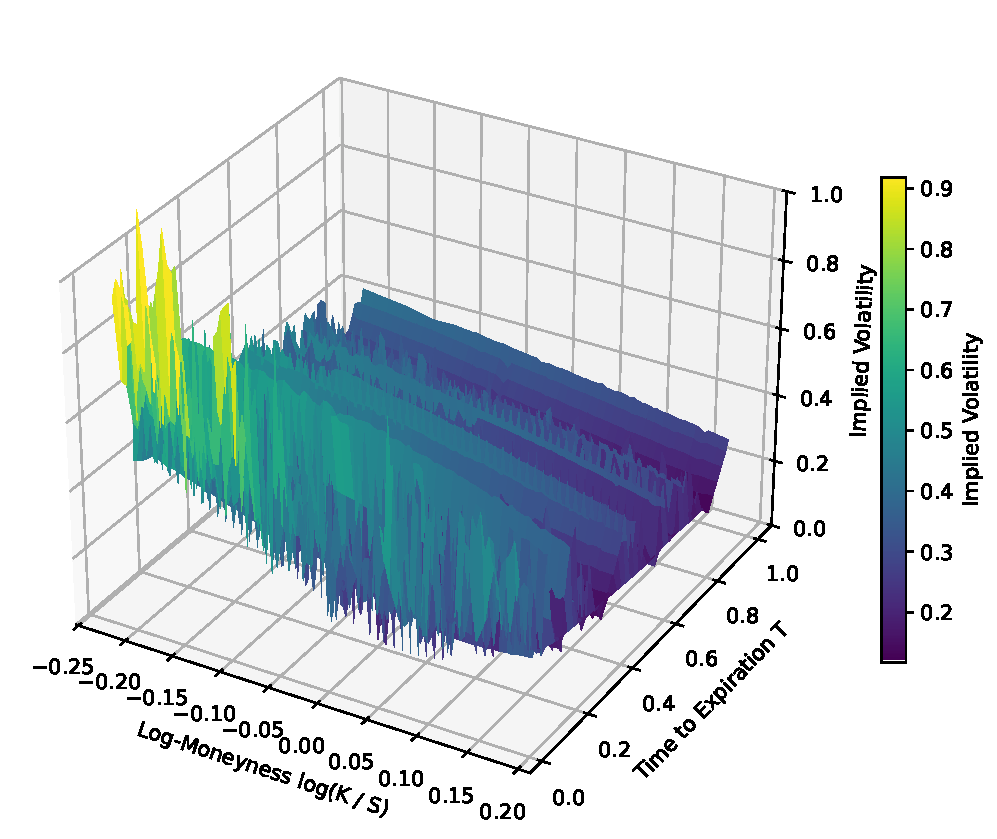
\includegraphics[width=\linewidth]{Images/implied_volatility_surface.pdf}

      \small Implied volatility surface
      \[
        \sigma_{\mathrm{imp}}(K,T)
      \]
    \end{column}

    \begin{column}{0.24\textwidth}
      \centering
      \Large
      \[
        \Longrightarrow
      \]
      \scriptsize
      \[
        \sigma_{\mathrm{loc}}^2(K,T)
        =
        \frac{\frac{\partial C}{\partial T}
        + rK\frac{\partial C}{\partial K}}
        {\frac{1}{2}K^2\frac{\partial^2 C}{\partial K^2}}
      \]
    \end{column}

    \begin{column}{0.38\textwidth}
      \centering
      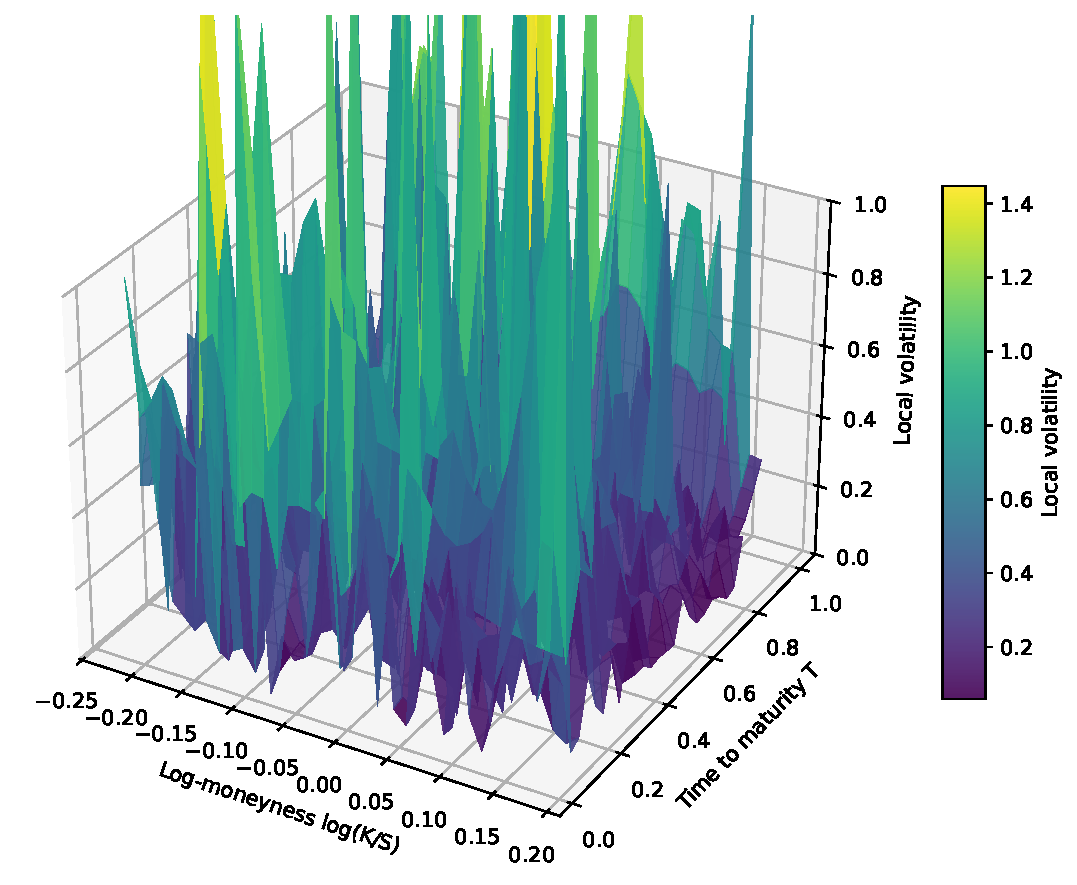
\includegraphics[width=\linewidth]{Images/local_volatility_surface.pdf}

      \small Local volatility surface
      \[
        \sigma_{\mathrm{loc}}(S,t)
      \]
    \end{column}
  \end{columns}
\end{frame}

\begin{frame}{Delta Proxy for Hedging}
  \begin{itemize}
    \item A fully model-consistent Dupire delta would price the option under
    local-volatility dynamics and then compute
    \[
      \Delta_{\mathrm{Dupire}} = \frac{\partial V}{\partial S}.
    \]
    \item In our implementation, we use a practical proxy: look up
    $\sigma_{\mathrm{loc}}(S,t)$ and plug it into the Black--Scholes delta formula.
    \[
      \Delta_{\mathrm{proxy}}
      =
      N\!\left(
      \frac{\log(S/K) + \left(r+\frac{1}{2}\sigma_{\mathrm{loc}}^2\right)T}
      {\sigma_{\mathrm{loc}}\sqrt{T}}
      \right).
    \]
    \item This gives a fast, interpretable hedge ratio for daily rebalancing.
    \item As a check, a finite-difference Monte Carlo Dupire delta gave a similar
    order of magnitude: $0.47$ versus proxy value $0.54$ for the ATM example.
  \end{itemize}
\end{frame}

\begin{frame}{Interpretation and Limitations}
  \begin{itemize}
    \item Under ideal smooth, arbitrage-free data, Dupire calibrates exactly to the observed call price surface.
    \item It turns market-implied option prices into a dynamic stock-price model for pricing and hedging.
    \item In practice, data are finite and noisy: missing quotes, bid-ask spreads, and interpolation matter.
    \item The formula uses numerical derivatives, so noise can be amplified.
    \item This motivates smoother approximations and learning-based methods, which the next section considers.
  \end{itemize}
\end{frame}

\end{document}
